%%%%%%%%%%%%%%%%%%%%%%%%%%%%%%%%%%%%%%%%%%%%%%%%%%%%%%%%%%%%%%%%%%%%%%%%%%%%%%%%%%%%
% Document data
%%%%%%%%%%%%%%%%%%%%%%%%%%%%%%%%%%%%%%%%%%%%%%%%%%%%%%%%%%%%%%%%%%%%%%%%%%%%%%%%%%%%
\documentclass[12pt]{article} %report allows for chapters
%%%%%%%%%%%%%%%%%%%%%%%%%%%%%%%%%%%%%%%%%%%%%%%%%%%%%%%%%%%%%%%%%%%%%%%%%%%%%%%%%%%%
\usepackage{preamble}

\begin{document}

\begin{center}
   \textsc{\large MATH 271, Homework 6, \emph{Solutions}}\\
   \textsc{Due October 18$^\textrm{th}$}
\end{center}
\vspace{.5cm}

\begin{problem}
Consider the differential equation
\[
f'(x) = \frac{1}{\sqrt{1-x^2}} f(x).
\]
\begin{enumerate}[(a)]
    \item Write down the 2$^\textrm{nd}$ order Taylor approximation to $\frac{1}{\sqrt{1-x^2}}$ centered at zero.
    \item Using this second order approximation, find the general solution to the differential equation using separation.
    \item The solution you find using the approximation doesn't have an issue at $x=1$, but I claim the original equation does.  What is wrong at $x=1$? Our approximation is then only reasonable in the window $[0,1)$ (and really isn't that accurate near 1 either).
\end{enumerate}
\end{problem}
\begin{solution}~
\begin{enumerate}[(a)]
    \item We need only compute up to the second derivative of $\frac{1}{\sqrt{1-x^2}}$ to get the desired approximation.  So we have
    \begin{align*}
        f^{(0)}(x)&= \frac{1}{\sqrt{1-x^2}} &&& \implies ~f^{(0)}(0)&=1\\
        f^{(1)}(x)&= \frac{x}{\left(1-x^2\right)^{3/2}} &&& \implies~ f^{(1)}(0)&=0\\
        f^{(2)}(x)&= \frac{3x^2}{\left(1-x^2\right)^{5/2}} + \frac{1}{\left(1-x^2\right)^{3/2}} &&& \implies ~f^{(2)}(0)&=1.
    \end{align*}
    Hence we have that
    \[
    \frac{1}{\sqrt{1-x^2}} \approx 1+\frac{x^2}{2}
    \]
    to second order.
    \item Now the approximate equation is
    \[
    f'(x)\approx \left(1+\frac{x^2}{2}\right)f(x)
    \]
    which we can solve using separation.  Thus,
    \begin{align*}
        \frac{1}{f}df&=\left(1+\frac{x^2}{2}\right)dx\\
        \ln(f)&= x+\frac{x^3}{6}+C\\
        \implies ~ f&= Ce^{x+\frac{x^3}{6}}.
    \end{align*}
    \item As $x\to 1^-$ in the above equation, we have that the right hand side may approach infinity since 
    \[
    \lim_{x\to 1^-} \frac{1}{1-x^2}=\infty.
    \]
    Now, if $f(x)\to 0$ quickly enough, it could be that these effects mitigate each other to some extent, but this is not the case.  We have that if $f(0)=0$, then the solution is stationary. If $f(0)>0$ the solution will grow to infinity by the point $x=1$ since $f(x)$ and $f'(x)$ will both be positive we already showed the above limit.  Similarly, if $f(0)<0$, then the solution grows to negative infinity by the point $x=-1$ for analogous reasons.  
    \begin{figure}[H]
        \centering
        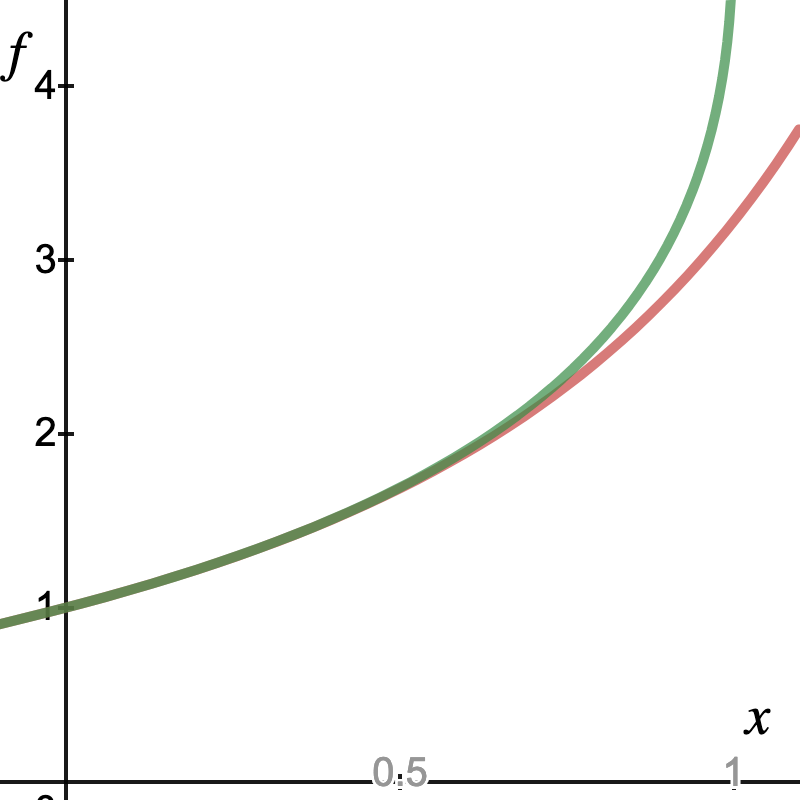
\includegraphics[width=.5\textwidth]{desmos-graph.png}
        \caption{A graph of the true solution (green), and approximate solution (red).}
    \end{figure}
    \end{enumerate}
\end{solution}

\newpage
\begin{problem}
Consider the differential equation
\[
f'(x)=xf(x)
\]
with initial condition $f(0)=1$.  
\begin{enumerate}[(a)]
    \item Find the particular solution to this differential equation using separation.
    \item What is the Taylor series centered at zero for this solution?
    \item Now, assume that the solution $f(x)$ can be written as a power series
    \[
    f(x) = \sum_{n=0}^\infty a_n x^n.
    \]
    Determine all of the coefficients $a_n$ which will give us the power series representation for $f(x)$. \emph{Hint: use your solution from (a) to help you.}
\end{enumerate}
\end{problem}
\begin{solution}~
\begin{enumerate}[(a)]
    \item Using separation,
    \begin{align*}
        f'&=xf\\
        \frac{1}{f}df&=xdx\\
        \ln(f)&= \frac{x^2}{2}+C\\
        f&= Ae^{\frac{x^2}{2}}.
    \end{align*}
    Then with $f(0)=1$, we have
    \[
    1=A,
    \]
    so the particular solution is
    \[
    f(x)=e^{\frac{x^2}{2}}.
    \]
    \item Note that we have
    \[
    e^{x}=\sum_{n=0}^\infty \frac{x^n}{n!}
    \]
    and thus
    \[
    e^{\frac{x^2}{2}}= \sum_{n=0}^\infty \frac{ \left( \frac{x^2}{2}\right)^n}{n!} = \sum_{n=0}^\infty \frac{x^{2n}}{2^nn!}.
    \]
\end{enumerate}
\item Now, to solve this using a power series, we assume the ansatz that $f(x)$ takes the form
\[
f(x)=\sum_{n=0}^\infty a_nx^n.
\]
Then we also have
\[
f'(x)=\sum_{n=1}^\infty na_n x^{n-1},
\]
and we can plug both series into the original equation to get
\begin{align*}
    \sum_{n=1}^\infty na_n x^{n-1} &= x \sum_{n=0}^\infty a_nx^n\\
    \sum_{n=1}^\infty na_nx^{n-1}&= \sum_{n=0}^\infty a_nx^{n+1}.
\end{align*}
So we can solve for the coefficients $a_n$ to determine $f(x)$,
\begin{align*}
    \sum_{n=1}^\infty na_nx^{n-1}&= \sum_{n=0}^\infty a_nx^{n+1}\\
    \sum_{n=0}^\infty (n+1)a_{n+1} x^n - \sum_{n=1}^\infty a_{n-1}x^n &=0\\
    a_1 + \sum_{n=1}^\infty \left[ (n+1)a_{n+1} - a_{n-1}\right]x^n &=0.
\end{align*}
Hence we must have that $a_1=0$ and that
\[
(n+1)a_{n+1}-a_{n-1}=0,
\]
which means that
\[
a_{n+1}= \frac{1}{n+1} a_{n-1}.
\]
Since $a_1=0$, we have that all odd terms $a_{2n+1}=0$ by the above relationship. Then we have for the even terms
\begin{align*}
    a_2 &= \frac{1}{2} a_0 = \frac{1}{2^1}\cdot \frac{1}{1!}a_0\\
    a_4 &= \frac{1}{4} a_2 = \frac{1}{4}\cdot \frac{1}{2} a_0 = \frac{1}{2^2}\cdot \frac{1}{2!}a_0\\
    a_6 &= \frac{1}{6}a_4 = \frac{1}{6}\cdot \frac{1}{4}\cdot \frac{1}{2}a_0 = \frac{1}{2^3} \cdot \frac{1}{3!}a_0\\
    &\vdots\\
    \implies~a_{2n}&= \frac{1}{2^n}\cdot \frac{1}{n!} a_0.
\end{align*}
Hence our general solution is
\[
f(x)=a_0 \sum_{n=0}^\infty \frac{x^{2n}}{2^n n!}.
\]
If we require that $f(0)=1$, then $a_0=1$ and we have
\[
f(x)=\sum_{n=0}^\infty \frac{x^{2n}}{2^n n!},
\]
which is exactly what we found in (b).
\end{solution}


\newpage
\begin{problem}
Consider the differential equation
\[
(x-1)f'(x) + f(x)=0
\]
with initial condition $f(0)=1$.
\begin{enumerate}[(a)]
    \item Find the solution to this equation using separation.
    \item Find the Taylor series centered at zero for your solution in (a).
    \item Again, suppose that the solution can be written as a power series and determine all the coefficients $a_n$ so that we find the power series representation for $f(x)$. \emph{Hint: use your solution from (a) to help you.}
\end{enumerate}
\end{problem}
\begin{solution}~
\begin{enumerate}[(a)]
    \item Using separation,
    \begin{align*}
        f'&=\frac{1}{1-x}f\\
        \frac{1}{f}df&=\frac{1}{1-x}dx\\
        \ln(f)&= -\ln(1-x)+C\\
        f&= \frac{A}{1-x}.
    \end{align*}
    Then with $f(0)=1$, we have
    \[
    1=A,
    \]
    so the particular solution is
    \[
    f(x)=\frac{1}{1-x}.
    \]
    \item Note that $f(x)$ is the result of the geometric series so that
    \[
    \frac{1}{1-x}=\sum_{n=0}^\infty x^n.
    \]

\end{enumerate}
\item Now, to solve this using a power series, we assume the ansatz that $f(x)$ takes the form
\[
f(x)=\sum_{n=0}^\infty a_nx^n.
\]
Then we also have
\[
f'(x)=\sum_{n=1}^\infty na_n x^{n-1},
\]
and we can plug both series into the original equation to get
\begin{align*}
    (x-1)\sum_{n=1}^\infty na_n x^{n-1} +  \sum_{n=0}^\infty a_nx^n = 0\\
    \sum_{n=1}^\infty na_n x^{n}-\sum_{n=1}^\infty na_n x^{n-1} +  \sum_{n=0}^\infty a_nx^n = 0\\
    \sum_{n=1}^\infty na_n x^{n}-\sum_{n=0}^\infty (n+1)a_{n+1} x^{n} +  \sum_{n=0}^\infty a_nx^n = 0,
\end{align*}
where we reindexed in the last line. To determine the coefficients $a_n$, we combine terms and extrude the first terms to get
\begin{align*}
    a_0- a_1 + \sum_{n=1}^\infty [na_n -(n+1)a_{n+1}+a_n]x^n =0.
\end{align*}
Hence we must have that $a_0 - a_1=0$ so $a_0=a_1$ and the other coefficients must be zero so
\[
0n a_n - (n+1)a_{n+1} + a_n = (n+1)(a_n-a_{n+1}), 
\]
which means that
\[
a_{n+1}= a_n
\]
Thus, all the coefficients are equal to one another and in particular $a_n=a_0$. Hence our general solution is
\[
f(x)=a_0 \sum_{n=0}^\infty x^n.
\]
If we require that $f(0)=1$, then $a_0=1$ and we have
\[
f(x)=\sum_{n=0}^\infty x^n,
\]
which is exactly what we found in (b).
\end{solution}

\newpage
\begin{problem}
We derived two linearly independent (even and odd) solutions to \emph{Legendre's equation}
\[
(1-x^2)f''(x)-2xf'(x)+l(l+1)f(x)=0
\]
which were
\[
f(x)=\sum_{n=0}^\infty a_{2n}x^{2n} \qquad \textrm{and} \qquad f(x)=\sum_{n=0}^\infty a_{2n+1}x^{2n+1}.
\]
\begin{enumerate}[(a)]
    \item Look up where this equation shows up in quantum mechanics and write it down.
    \item If we add initial conditions then we get a finite polynomial for each choice of $\alpha = 0,1,2,3,\dots$. Using this, the first four polynomials are
    \begin{align*}
        f_0(x)&=1 &&& f_1(x)&=x\\
        f_2(x)&=1-3x^2 &&& f_3(x)&=x-\frac{5x^3}{3}.
    \end{align*}
    Show that these above polynomials are \emph{orthogonal} by showing
    \[
    \int_{-1}^1 f_i(x)f_j(x)dx = 0 
    \]
    when $i\neq j$.
\end{enumerate}
\end{problem}
\begin{solution}~
\begin{enumerate}[(a)]
    \item This equation arises in quantum mechanics when solving for the solution to the Hydrogen atom.  Specifically, one finds the differential equation
    \[
    \frac{d^2y}{d\theta^2} + \frac{\cos \theta}{\sin \theta} \frac{dy}{d\theta} + \left[ (l(l+1)-\frac{m^2}{\sin^2 \theta} \right]y =0.
    \]
    If we take $m=0$ in the above equation, then we arrive at the Legendre equation provided above, but in the variable $x=\cos\theta$.  This variable represents the polar angle part of the solution found using separation of variables for the central Coulomb potential for a proton and electron (i.e., the Hydrogen atom).
    \item We simply have to compute integrals for the following pairs of $(i,j)$:
    \[
    (0,1) \quad (0,2) \quad (0,3) \quad (1,2) \quad (1,3) \quad (2,3).
    \]
    We compute each
    \begin{align*}
        \int_{-1}^1 f_0(x)f_1(x)dx &= \int_{-1}^1 1\cdot x dx \\
        &=0,
    \end{align*}
    since $x$ is an odd function on a symmetric interval about $x=0$.
    
    Next, we take
    \begin{align*}
        \int_{-1}^1 f_0(x)f_2(x) dx &= \int_{-1}^1 1\cdot (1-3x^2)dx\\
        &= \int_{-1}^1 dx - 3 \int_{-1}^1 x^2 dx\\
        &= 2 - \left[ x^3\right]_{-1}^1 \\
        &= 0.
    \end{align*}
    
    Next,
    \begin{align*}
        \int_{-1}^1 f_0(x) f_3(x) dx &= \int_{-1}^1 1 \cdot \left( x-\frac{5x^3}{3}\right)dx\\
        &= 0,
    \end{align*}
    since $f_3(x)$ is an odd function. 
    
    Next,
    \begin{align*}
        \int_{-1}^1 f_1(x)f_2(x)dx&= \int_{-1}^1 x\cdot \left(1-3x^2\right) dx\\
        &=0,
    \end{align*}
    since $f_1(x)$ is an odd function and $f_2(x)$ is an even function and an even function times an odd function is an odd function.
    
    Next,
    \begin{align*}
        \int_{-1}^1 f_1(x)f_3(x)dx &= \int_{-1}^1 x\cdot \left( x-\frac{5x^3}{3}\right)dx\\
        &= \int_{-1}^1 x^2 dx - \frac{5}{3}\int_{-1}^1 x^4 dx \\
        &= \frac{2}{3} - \frac{5}{3}\cdot \frac{2}{5}\\
        &=0.
    \end{align*}
    
    Lastly, we take
    \begin{align*}
        \int_{-1}^1 f_2(x) f_3(x)dx &= \int_{-1}^1 \left(1-3x^3\right) \cdot \left( x-\frac{5x^3}{3}\right)\\
        &=0,
    \end{align*}
    again since the product of an even and odd function is odd. Hence, we have shown the orthogonality relationship between all the relevant functions.
\end{enumerate}
\end{solution}
\end{document}